% This file should be replaced with your file with an thesis content.
%=========================================================================
% Authors: Michal Bidlo, Bohuslav Křena, Jaroslav Dytrych, Petr Veigend and Adam Herout 2019

\hyphenation{OpenStack Swift OpenIO SDS}

\chapter{Introduction}

% general introduction for a topic:
%- cloud computing popularity
%- most popular service: cloud storage and its types
%- about object storage
%- users interest of what's going in theirs storage / event activities
%- TODO: maybe remove talk about types of cloud storages? solution: talk about need for monitoring and users need to monitor/receive information regarding their storage
In the current world, cloud computing became the most popular way of delivering different types of services throught Internet. One of the most popular cloud service is cloud storage, which allows users to store data in remote locations mentained by third party. Based on how cloud storage manages data, cloud storage can be divided into 3 types: Block storage, File storage and Object storage. Object storage manages data as objects, each object typically includes data itself and some additional informations stored in objects metadata. Since data are stored in remote locations, to which users don't have direct and complete access, some users or external services might want to receive informations about certain events (for example change of content) in storages where their data are located.

% importance of thesis in this field
%- react to events - possibly react to 'bad' events
%- allows users to have better picture what is going on in their storage
Importance of this thesis is to provide event informations to users in OpenIO SDS and OpenStack Swift, which will allow user to react on those events and possibly prevent/detect unwanted actions. Providing event notifications will allow users to have better picture on what is going on in their storage and impove monitoring in these object storages.

%past advances in this field
There was two attempts\cite{swiftPatch1}\cite{swiftPatch2} to solve this issue within OpenStack Swift which were not officially accepted and their solution is outdated. Currently there is no official solution for publishing event notification in OpenStack Swift nor OpenIO Software-Defined Storage (hereinafter SDS).

%why am I interested in this, why I choose this topic
%- perosnally i used object storage
%- can se myself using this solution in future as well as millions of other users
%- impact on big amount of users
%- contibuting to open source projects
My interest in this topic steems from its possible impact to extensive amount of users that OpenStack Swift and OpenIO have. Contibuting to open source projects is something that I always wanted to be part of. Possiblity to improve user experience in OpenStack Swift and OpenIO SDS and allow those storages to be even more competative against comercial storages (Amazon, Google, ...) is another reason why I choose this topic.

%goals of thesis
The goal of this thesis is to create program/middleware which wil publish event notification to user specified destination. One of supported destination will be Beanstalk queue, but program will allow to easily add other types of destinations (for example Kafka) using predefined interface. Proposed program will allow user to specify, using objects metadata (such as name prefix/sufix and object size) and type of event, which event notification should be published. Program will be able to run within OpenStack Swift as well as OpenIO SDS. This thesis will strive to find such solution that could be officially accpeted as part of OpenStack Swift and OpenIO SDS.

%structure of thesis
Structure of thesis - TODO - there will be probably change in chpaters structure

\chapter{Background}

This chapter introduces Object storage, its core concepts, and the underlying technologies. After introducing the Object storage, for sufficient understanding of this master thesis topic, it is essential to explain how Software-defined storage manages data, and what types of events can occur inside. The last part of this chapter describes the concept of event notifications, why they are essential, and current interfaces for publishing them to users.

\section{Object storage}
    %introduction/concept
    Object storage, also known as \textit{object-based storage (OBS)}, handles data as objects instead of hierarchical methods used in file systems\cite{objectBasedStorage}. The object storage is designed to handle data as whole objects, making it an ideal solution for any unchanging data. Data in object stores are changed by replacing objects or files, and therefore object stores are the preferred mechanism for storing such files\cite{networkStorage}.

    %key koncepts
    %-metadata are stored in same object store device but on separated location
    \subsection{Key concepts}
    Key concepts of object storage are\cite{ibmObjectStorage}:
    \begin{itemize}
        \item Objects - An object typically consist of user data and metadata uploaded to object storage.
        \item Containers/Buckets - represents logical abstraction used to provide a data container in object storage. An object with the same name in two different containers represents two different objects. This concept segregates data using bucket ownership and a combination of public and secret keys bound to object storage accounts, allowing users and applications to manipulate with authorized data for specific types of manipulation (read/write/update).
        \item Metadata - Additional information about data, such as date of creation and last modification, size, hash.
        \item Access Control Lists(ACLs) - used as primary security construct in object storage, stored in account or bucket level and allows owners to grant permissions for certain operations based on UUID, email, ...
        \item Object Data protection - two primary data protection schemes in object storage are Replication and Erasure Coding.

        \textbf{Replication} is a method used to ensure data resilience. Data are copied into multiple locations/disks/partitions. In case of failure, data are used from a secondary copy to recreate the original copy or as a primary copy.

        \textbf{Erasure coding} is a process through which the data is separated into fragments. Then fragments are expanded and encoded with redundant pieces and stored across different storage devices. Erasure coding adds redundancy and allows object storage to tolerate failures.
    \end{itemize}


    \subsection{Object data}
    %types of stored informations
    With object storage techniques, each object contains\cite{ibmObjectStorage}:
    \begin{itemize}
      \item \textbf{Data} - user-specified data that needs to be stored in persistent storage. Such data can be binary data, text file, image, etc.
      \item \textbf{Metadata} - additional data that describe objects data. Metadata can be divided into two types: Device-managed metadata is additional information maintained by a storage device and used as part of object management in physical storage\cite{objectBasedStorage}. The second type is Custom metadata, to which users can store any additional information in key and value pairs. In object storage, metadata is stored together with the object.
      \item \textbf{A universally unique identifier (UUID)} - This ID, created using a hashing process based on object name and other additional information, is assigned to each object in object storage. Using ID object storage systems can tell apart objects from one another. ID is also used to extract data in a system without knowing their physical location/drive and offset.
    \end{itemize}

    \subsection{Access to object storage}
    %access to object storage
    %-resfull interface
    %-advantages of this approach
    %-popular intefaces
    Object storage services provide a RESTful interface \cite{cloudObjectStorage} over HTTP protocol to store and access objects. This approach allows users to create, read, delete, update, or even query objects anytime and anywhere simply by referencing UUID (or using specific attributes for querying), usually with a proper authentication process. The most popular interfaces for communicating with object storages are Amazon S3 (Simple Storage Service) API and OpenStack Swift API.

    %comparison to other storage models
    \subsection{Pros and cons of object storage}
    Pros:
    \begin{itemize}
        \item Capable of handling a large amount of unstructured data
        \item Reduced TCO and cheap COTS - Object storage is designed to utilize cheap COTS(Commercial off-the-shelf) components. As a result Total Cost of Ownership(TCO) is lower than owning homemade Network-Attached Storage(NAS)\cite{networkStorage}.
        \item Unlimited scalability - Since object storages are built on distributed systems, they scale very well compared to traditional storages, where they often have an upper limit\cite{swiftEssentials}.
        \item Wide-open metadata - allows users to store custom metadata and the possibility of creating metadata-driven policies, such as compression and tiering.
    \end{itemize}
    Cons:
    \begin{itemize}
        \item No in-place update - object must be manipulated as a whole unit.
        \item No locking mechanism - object storage does not manage object-level locking, and it is up to applications to solve concurrent PUT/GET.
        \item Slower - this makes object storages a poor choice for applications that need rapid and frequent access to data.
    \end{itemize}

\section{Software-Defined storage}
    %introduction to topic
    Software-Defined Storage(SDS) is a storage architecture that separates software storage from hardware allowing greater scalability, flexibility, and control over the data storage infrastructure. With the growth of Software-Defined Networks(SDN) and the need for Software-Defined Infrastructure(SDI), which aims to virtualize network resources and separate control plane from the data plane, this principle was needed to be applied on Object storage as well\cite{sdsSDSMultiTenantEnv}.

    To overcome limitations of traditional storage infrastructures, the Software-Defined Storage (SDS) is imposed as a proper solution to simplify data and configuration management while improving the end-to-end control functionality of conventional storage systems\cite{sdsSurvey}. Furthermore, while traditional storages like storage area networks (SAN) and network-attached storage (NAS) provides scalability and reliability, SDS provides it with much lower cost by utilizing industry-standard or x86 system and therefore removing dependency on expensive hardware\cite{sdsWPRedHatSDS}.

    %principles
    % - Scale-out
    % - Customizable
    % - Automation
    % - Masking
    % - Policy Management
    \subsection{Principles}
    There is no clear definition on criteria for defining software-defined storage, although several fundamental principles can be deducted\cite{sdsGPCloudStorage}:
    \begin{itemize}
        \item \textbf{Scale-out} - SDS should enable low-cost horizontal scaling (by adding new commodity hardware to existing infrastructure) compared to vertical scaling with more powerful (and expensive) hardware.
        \item \textbf{Customizable} - SDS should offer system storage customization to meet specific storage QoS requirements. This will allow users to choose storage solution based on their requirements/performance and avoid unnecessary overpaying.
        \item \textbf{Automation} - once QoS is defined process of deployment and monitoring on object storage should be automated and done without the need for human resources.
        \item \textbf{Masking} - SDS can mask underlying storage system and distributed system as long as they provide common storage API and meet required QoS. SDS can offer block or File API even though data are saved in object storage (like Ceph does).
        \item \textbf{Police Management} - SDS Software must manage storage according to specified policies and QoS requirements despite being in multi-tenant space. SDS must be capable of handling failures and autoscale in case of change in workloads.
    \end{itemize}


    %architecture
    %   - data plane
    %   - control plane
    %functions
    %benefits
    \subsection{Architecture}
    As previously described, the main characteristic of SDS is to separate storage functions into control plane and data plane.

    \paragraph{Control plane}
    - the control plane represents an abstraction layer with main goal to virtualize storage resources. It offers high-level functions that are needed by the customer to run the business workload and enable optimized, flexible, scalable, and rapid provisioning storage infrastructure capacity. These capabilities span functions like policy automation, analytics and optimization, backup and copy management, security, and integration with the API services, including other cloud provider services\cite{sdsIBMSDSGuide}.

    \paragraph{Data plane}
    - the data plane encompasses the infrastructure where data is processed. It consists of all basic storage management functions, such as virtualization, RAID protection, tiering, copy services (remote, local, synchronous, asynchronous, and point-in-time), encryption, compression, and data deduplication that can be requested by the control plane. The data plane is the interface to the hardware infrastructure where the data is stored. It provides a complete range of data access possibilities and spans traditional access methods, such as block I/O (for example, iSCSI), File I/O (NFS, SMB, or Hadoop Distributed File System (HFDS)), and object-storage\cite{sdsIBMSDSGuide}.

    %todo image of layers from sdsSurvey
    \begin{figure}[hbt]
        \centering
        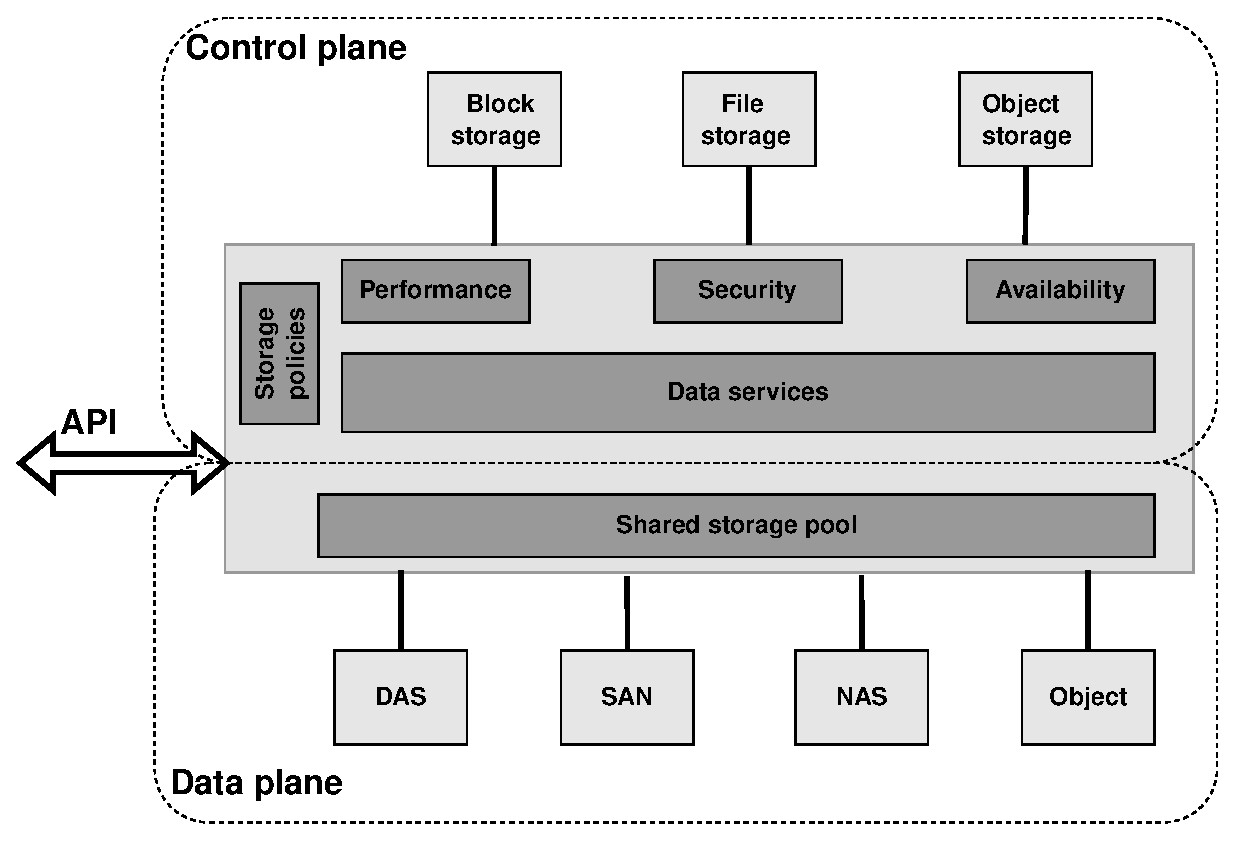
\includegraphics[width=1\textwidth]{obrazky-figures/sds-planes.eps}
        \caption{SDS data and control plane.\cite{sdsPlanes}, remade}
        \label{fig:beanstalkdJobSM}
    \end{figure}

\section{Beanstalk queue}

    Beanstalk queue or shorter beanstalkd is a fast, simple and lightweight working queue\cite{beanstalkdOfficial}. The primary use case is to manage workflow between different parts of workers of application through working queues and messages. Beanstalkd was developed for the need of Facebook application in order to reduce average response time\cite{beanstalkdOfficial}. Provided by simple protocol design, heavily inspired by Memcached, implemented in programming language C, Beanstalkd offers lean architecture, which allows it to be installed and used very simply, making it perfect for many use cases\cite{beanstalkdInstall}.


    \subsection{Beanstalkd elements}
    Beanstalkd is a priority queue with server-client architecture. The server represents queues where jobs are saved based on priority. Beanstalkd architecture is composed of several components:
    \begin{itemize}
        \item Jobs - tasks stored by the client
        \item Tubes - used for storing tasks, each tube contains a ready queue and a delay queue.
        \item Producer - creates and sends jobs to beanstalkd using command "put".
        \item Consumer - process "listening" on an assigned tube, reserves and consumes jobs from the tube.
    \end{itemize}

    \subsection{Job Lifecycle}
    Each job is uniquely assigned to one worker at a time. The client creates a job and inserts it to beanstalkd tube using "put" command. While being in the tube, the job can be in next states\cite{beanstalkdProtocol}:
    \begin{itemize}
        \item \textbf{Ready} - the task is free and can be executed immediately by the consumer.
        \item \textbf{Delayed} - the task has assigned delay time that needs to expire before execution. After delay time expires, beanstalkd will automatically change its state to READY.
        \item \textbf{Reserved} - the task is reserved and is being executed by the consumer. Beanstalkd is responsible for checking whether the task is completed in time (TTR - Time to run).
        \item \textbf{Buried} - reserved task, the task will not be removed nor executed until the client decides. This state is often used for further inspection in debugging process when failure or undefined behavior occurs during task execution.
        \item \textbf{Deleted} - the task is deleted from the tube, beanstalkd no longer maintains these jobs.
    \end{itemize}

    Figure \ref{fig:beanstalkdJobSM} describes the life cycle of a job in beanstalkd tube. Job is created by Producer using put command. Beanstalkd allows the Producer to add delay time before the task is ready for execution, setting the job state to DELAYED. After delay time expires, beanstalkd will automatically change job state to READY. The Producer can specify job priority and jobs with the READY state are stored in the priority queue. A job with the biggest priority is reserved and executed by a Consumer. After successfully executing the task, the Consumer will delete the job from beanstalkd. If some error occurs, the Consumer can bury the task. The Consumer can decide that he is not interested in completing the reserved task. Using the release command (with optional delay) job state will be changed back to READY (or DELAY). Jobs with the BURIED state will not be touched by beanstalkd server until the client "kicks" them to READY state.

    \begin{figure}[hbt]
        \centering
        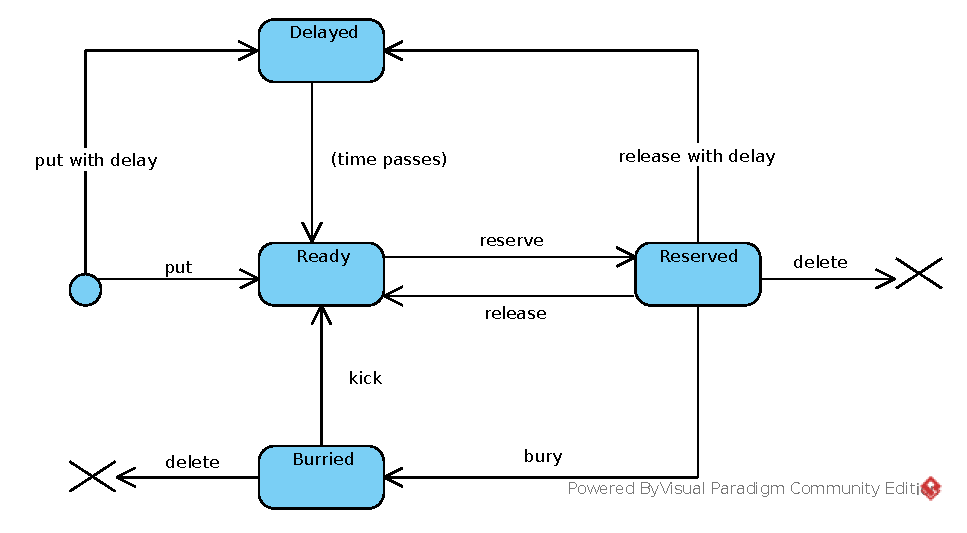
\includegraphics[width=1\textwidth]{obrazky-figures/beanstalkd-job-states.eps}
        \caption{State machine diagram of job in Beanstalkd tube}
        \label{fig:beanstalkdJobSM}
    \end{figure}


    \subsection{Key characteristics}
    Key beanstalkd characteristics are:

    \paragraph{Asynchronous}- beanstalkd allows producers to put jobs in the queue, and workers can process them later.
    \paragraph{Distributed}- in the same way as Memcached, beanstalkd can be distributed, although this distribution is handled by clients. The beanstalkd server does not know anything about other beanstalkd running instances.
    \paragraph{Persistent}- beanstalkd offers support for persistent jobs during which all jobs are written to binlog. In case of a power outage, after restarting beanstalkd instance, it will recover jobs content from the logs.
    \paragraph{Not secured}- beanstalkd is designed to be run in a private/secure network. Therefore it does not support authentication or authorization.
    \paragraph{Scalability}- beanstalkd can be scaled horizontally, although it must be done on the client side, where each client would connect to multiple servers and then use specific algorithms(e.g., Round-robin) to switch between the different servers.

\section{Event notifications}
    %introduction
    An \textit{event} is a runtime operation executed by a software element, representing a significant change or occurrence in a system. Event is created in order to make some information available to other software elements not specified by the operation\cite{eventArchitecturalPatterns}.

    \textbf{Event notification} is a message created by a system in orderto notify other parts of the system that an event has taken place\cite{eventRedHatEventDrivenArch}. Event notifications are usually used for monitoring and asynchronous job processing.

    In object storage, event notifications are used to notify users or tenants about specific changes and occurrences in their bucket or account. Typical event notifications include creating new (or updating existing) objects in the bucket. In addition, most object vendors offer Publish/subscribe notifications, allowing users to subscribe to certain types of event notifications using predefined rules. Information about rules specifying event notifications is usually stored in the upper-level metadata (bucket or account).

    \subsection{CloudEvents}
    Publishers tend to describe event data differently due to non-existing standards or formats. The lack of a common way to describe events means developers have to learn how to handle events for each event source. To solve this problem, CloudEvents was created.

    CloudEvents is a specification for describing event data in common way\cite{eventCloudEvents} hosted by Cloud Native Computing Foundation (CNCF)\cite{eventCNCF}. CloudEvents goal is to dramatically simplify event specification and delivery across services, platforms and beyond.
    CloudEvents has been integrated by many popular object storage vendors, such as Oracle Cloud, IBM Cloud Code Engine, Azure, Google Cloud etc.

    Attributes in CloudEvents specification can be divided into 3 categories:
    \paragraph{Required attributes} - set of attibures that are required to be included in all events\cite{eventCloudEventsSpec}:
    \begin{itemize}
        \item id (string) - event identifier, must not be empty.
        \item source (URI-reference) - identifies context in which event occured, must not be empty.
        \item specversion (string) - the version of CloudEvents specification, must not be empty.
        \item type (string) - value describing the type of occurred event. Often this attribute is used for policy enforcement, routing and monitoring.
    \end{itemize}

    \paragraph{Event data attirbutes} - attibures containing and describing event data:
    \begin{itemize}
        \item datacontenttype (string) - content type of data value (allows data to carry any type of content).
        \item dataschema (URI) - identifies the schema that data adheres to.
        \item data - data payload
    \end{itemize}

    \paragraph{Optional attributes}:
    \begin{itemize}
        \item time - timestamp
        \item subject (string) - the subject of the event in the context of the event producer.
        \item extension attributes - custom attibutes allowing external systems to attach metadata to an event.
    \end{itemize}

    \definecolor{darkpastelred}{rgb}{0.76, 0.23, 0.13}
    \lstset{
        string=[s]{"}{"},
        stringstyle=\color{darkpastelred},
        comment=[l]{:},
        commentstyle=\color{black},
        caption=Example of event described using CloudEvents specification and JSON
    }

    \begin{lstlisting}
    {
        "specversion" : "1.0",
        "type" : "com.github.pull_request.opened",
        "source" : "https://github.com/cloudevents/spec/pull",
        "subject" : "123",
        "id" : "A234-1234-1234",
        "time" : "2018-04-05T17:31:00Z",
        "comexampleextension1" : "value",
        "comexampleothervalue" : 5,
        "datacontenttype" : "text/xml",
        "data" : "<much wow=\"xml\"/>"
    }
    \end{lstlisting}

    \subsection{Amazon S3 event notifications}
    Amazon Simple Storage Service (S3) is one of the most popular cloud object storages providing a REST web service interface. Amazon S3 is reliable, scalable, commercial and one of the most popular object storage that manages Web-Scale computing by itself\cite{eventS3}. As a result, Amazon S3 has a big impact on object storage and most other object storage vendors crated compatible S3 API for their services.

    One of the monitoring features that Amazon S3 provides is Event Notification, which offers users to receive notifications when certain events happen in their S3 bucket. To enable such notifications, users need to create a notification configuration that identifies which events Amazon S3 should publish\cite{eventS3EventNotification}. Notifications are configured at the bucket level and then applied to each object in the bucket.

    Amazon S3 provides limited event destinations to which event notification messages can be send\cite{eventS3EventNotificationDest}:
    \begin{itemize}
        \item Amazon Simple Notification Service (Amazon SNS) - flexible, fully managed push messaging service, can be used to send messages to mobile phones or distributed services.
        \item Amazon Simple Queue Service (Amazon SQS) queues - reliable and scalable hosted queues for storing messages as they travel between computers.
        \item AWS Lambda - serverless, event-driven compute service. Lambda can run custom code in response to the Amazon S3 bucket event (if the lambda function writes to the same bucket that triggers the notification, it can create an execution loop).
        \item Amazon EventBridge - serverless event bus service used to receive events from AWS. It allows users to define rules to match events and deliver them to defined targets.
    \end{itemize}

    By this date, Amazon S3 does not support CloudEvents specification and describes event data in its own way. Some of event types that Amazon S3 can publish are\cite{eventS3EventNotificationDest}:


     \renewcommand*{\arraystretch}{1.4}
     \begin{tabularx}{\textwidth}{|p{0.3\textwidth}|X|}
         \hline
         \textbf{Event type} & \textbf{Desription} \\
         \hline
         s3:TestEvent & after enabling the event notifications, Amazon S3 publishes a test notification to ensure that topic exist and bucket owner has permissions to publish specified topic. \\
         \hline
         s3:ObjectCreated:* & An object was created (regardless on operation). \\
         \hline
         s3:ObjectCreated:Put & An object was created by an HTTP PUT operation. \\
         \hline
         s3:ObjectCreated:Post & An object was created by HTTP POST operation. \\
         \hline
         s3:ObjectCreated:Copy & An object was created an S3 copy operation. \\
         \hline
         s3:ObjectCreated:

         CompleteMultipartUpload & An object was created by the completion of a S3 multi-part upload. \\
         \hline
         s3:ObjectRemoved:* & An object was removed (regardless on operation). \\
         \hline
         s3:ObjectRemoved:Delete & An object was deleted by HTTP DELETE operation. \\
         \hline
         s3:ObjectRemoved:

         DeleteMarkerCreated & An versioned object was marked for deletion. \\
         \hline
    \end{tabularx}


\chapter{OpenIO SDS}
    OpenIO Software-defined storage is open source object storage that is perfectly capable of traditional use cases (such as archiving, big data, cloud). However, at the same time, combined with Grid for Apps (\ref{sec:oioGridForApps}), it opens the door for users to create an application that needs much more sophisticated back-end operations. These applications include industrial IoT, machine learning and artificial intelligence, as well as any other applications whose workflow can benefit from automated jobs or tasks\cite{oioNextGen}. In addition, OpenIO SDS is event-driven storage with the ability to intercept events seamlessly and transparently to the rest of the stack.

    \section{Key characteristics}
    \subsection*{Hardware agnostic}
    OpenIO SDS is fully software-defined storage capable of running on x86 or ARM hardware with minimal requirements. Cluster nodes can be different from each other, allowing different generations, types and capacities to be combined without affecting a performance or efficiency\cite{oioKeyChars}.
    OpenIO has built-in support for heterogeneous hardware allowing every node to be used at its maximum performance.
    \subsection*{No SPOF architecture}
    Every single service used to serve data is redundant from object chunks stored in a disc to the directory level, every information is duplicated. As a result, there is no single point of failure (SPOF) in the cluster and a node can be shutdown without affecting overall availability or integrity\cite{oioCoreSolution}.
    \subsection*{Cluster organization}
    Instead of a traditional cluster ring-like layout, OpenIO SDS is based on a grid of nodes \ref{fig:oioArch}. It is flexible and resource-conscious. Compared to other object storage solutions, cluster organization is not based on static data allocation that usually use Chord peer-to-peer distributed hash table algorithm. Instead, OpenIO SDS uses distributed directory for organizing data and metadata hash tables, which allows the software to attain the same level of scalability but with better and more consistent performance\cite{oioKeyChars}.

    \begin{figure}[hbt]
        \centering
        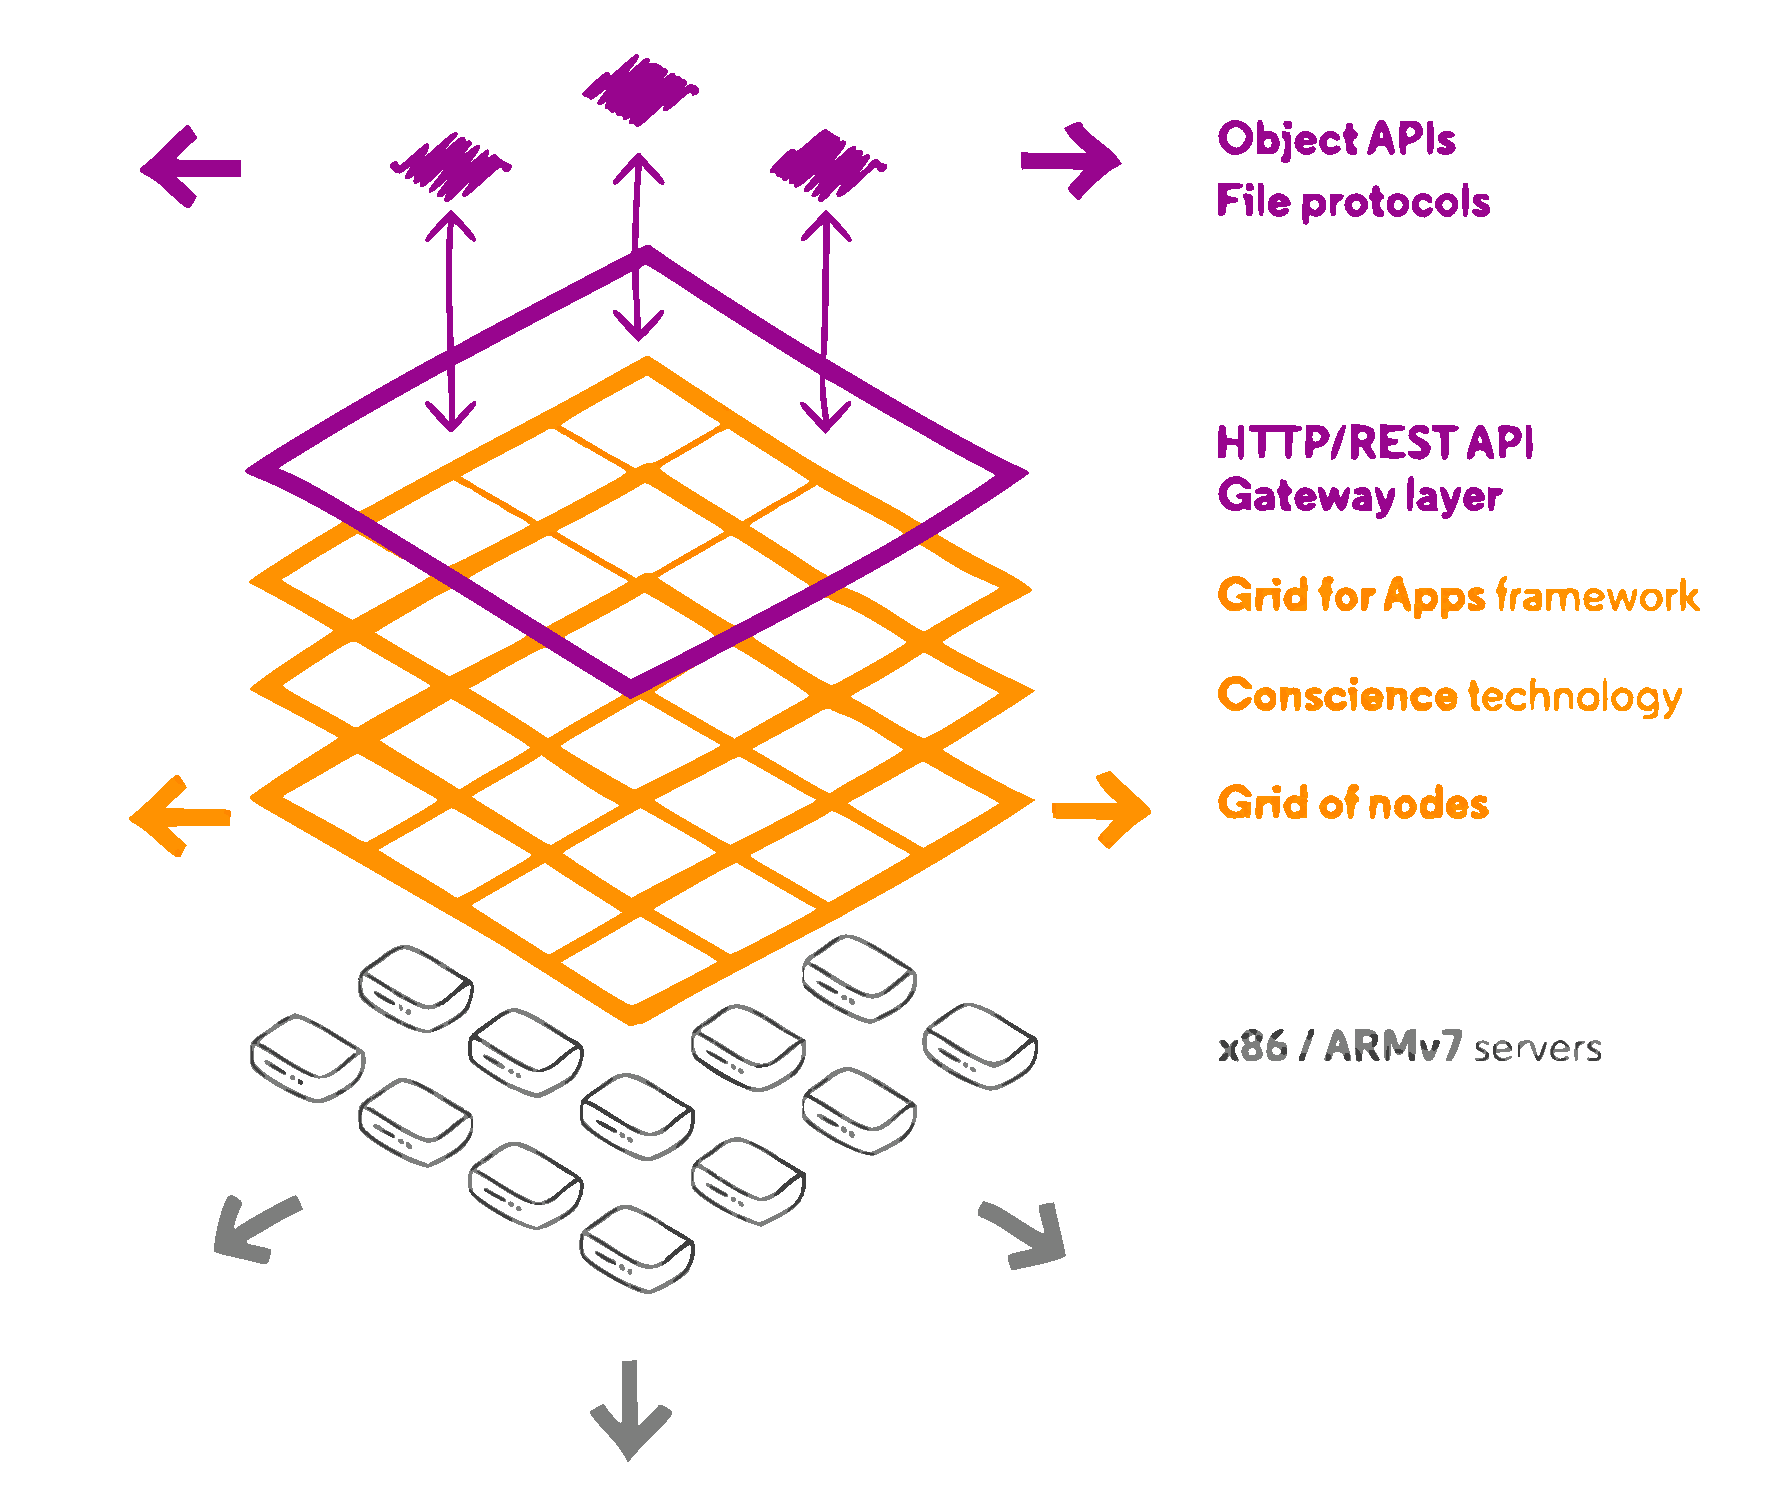
\includegraphics[width=1\textwidth]{obrazky-figures/openio-architecture.eps}
        \caption{Layered view on OpenIO SDS architecture.\cite{oioArch}}
        \label{fig:oioArch}
    \end{figure}


    \subsection*{Tiering}
    With tiering, OpenIO SDS offers users to configure a pool containing a group of hardware that can then be used to store specific types of objects. For example, users can create a pool of high-performance hard disks (e.g. SSDs) and use the pool to store objects that require low latency.
    This feature is realized by a mechanism called storage policies. Multiple storage policies can be defined in one particular namespace. Storage policies can also be used for specifying how many replicas should be created for a specific dataset\cite{oioCoreSolution}.

    \section{Data organization}
    Multi-tenancy is one of the core concepts in OpenIO SDS. Data objects are stored within following hierarchy: Namespace/Account/Container/Object \ref{fig:oioDataOrganization}. Multiple namespaces can be configured in each cluster, providing multi-region/zone logical layouts for applications and segregated workloads depending on a tenant or geo-distribution need\cite{oioSdsConcepts}.
    There is no classic subdirectory tree. Instead, objects are stored in a flat structure in the container level. However, like many other object storages, there is a way to emulate a filesystem.

    \begin{figure}[hbt]
        \centering
        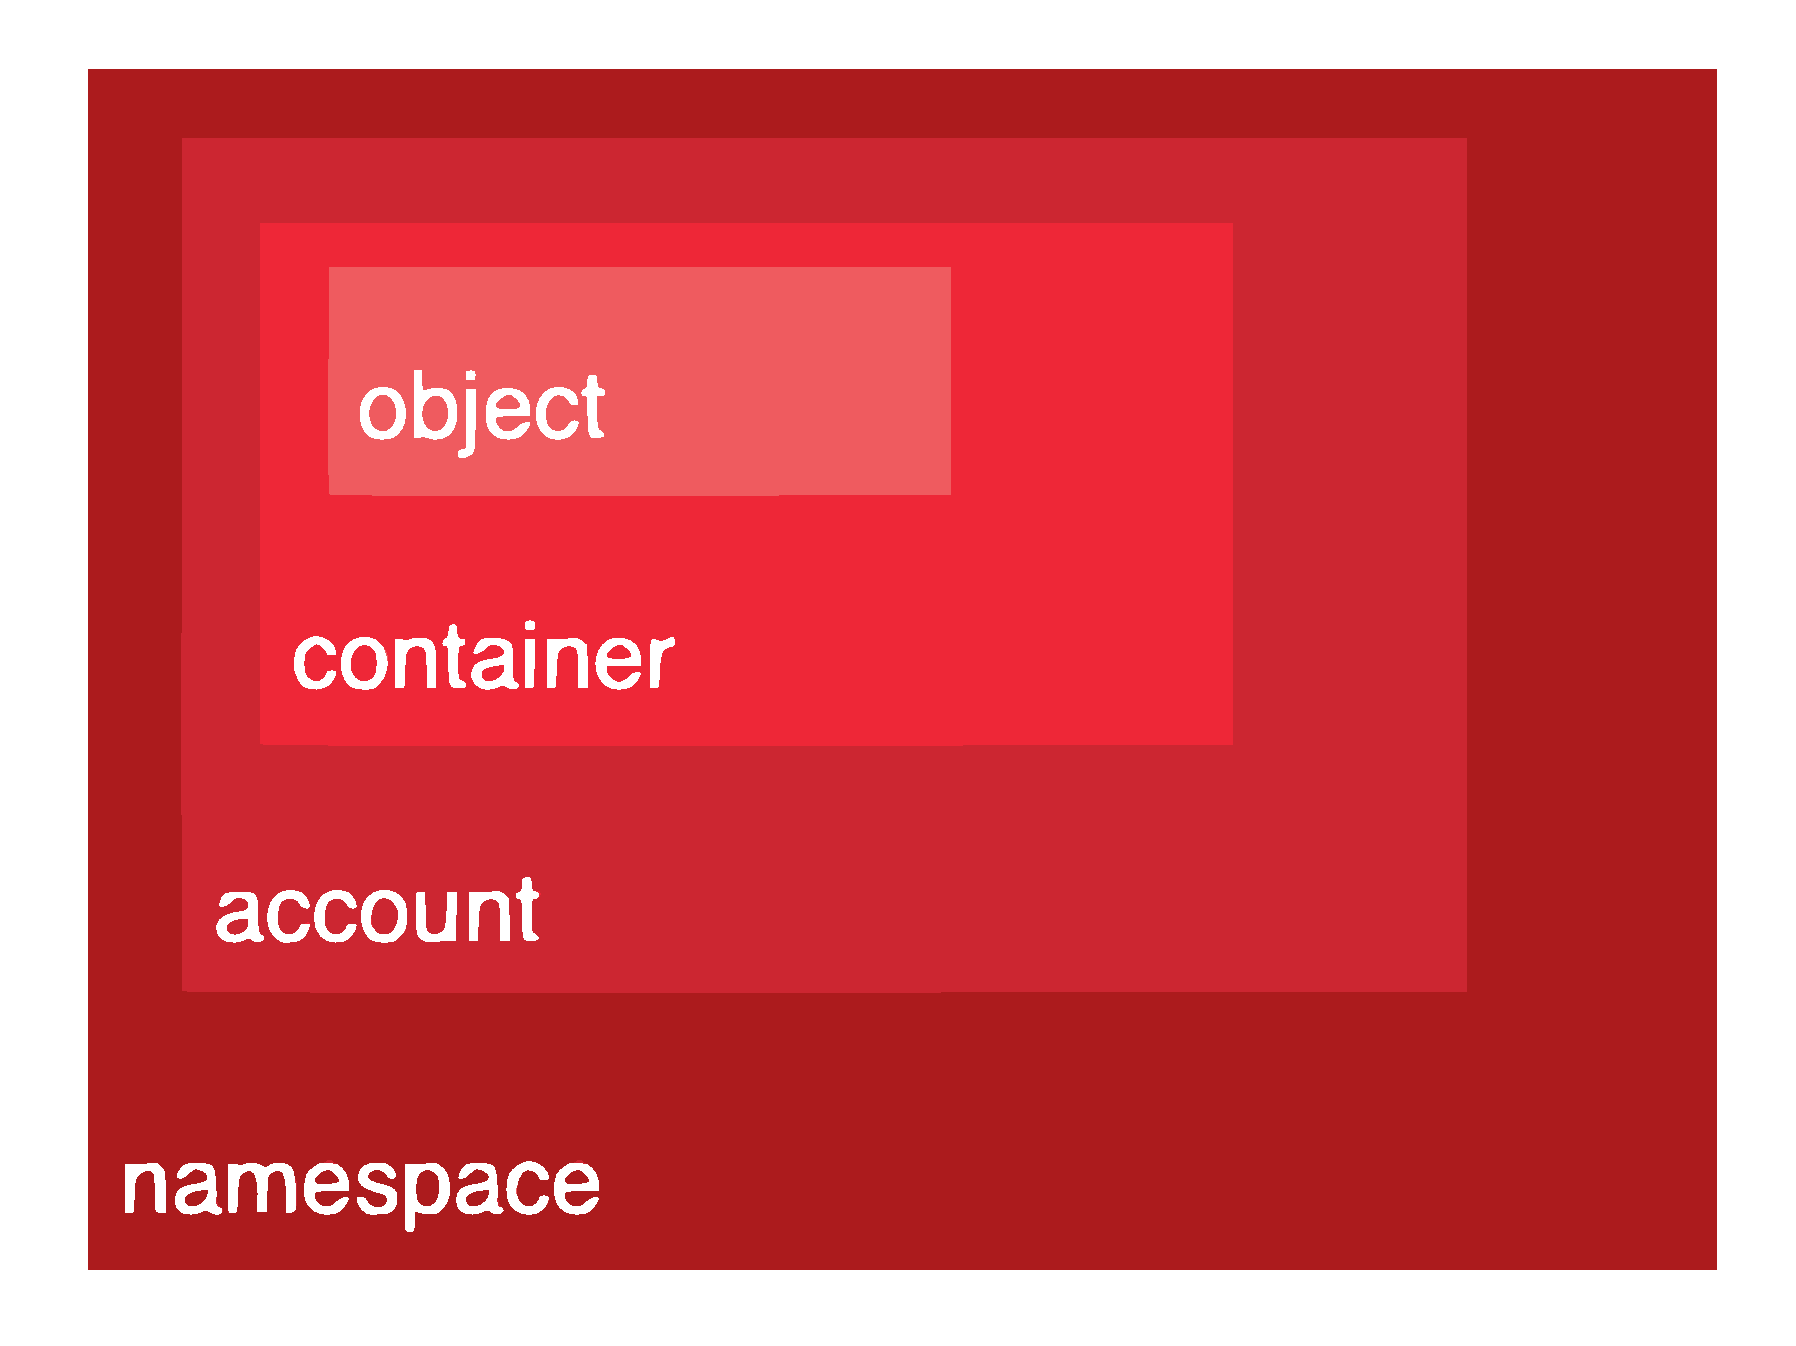
\includegraphics[width=0.5\textwidth]{obrazky-figures/openio-data-organization.eps}
        \caption{Object data organization in OpenIO SDS.\cite{oioCoreSolution}}
        \label{fig:oioDataOrganization}
    \end{figure}

    \subsection{Namespace}
    A coherent set of network services working together to run OpenIO's solutions. It hosts services and provides operations such as service configuration and monitoring.

    \subsection{Account}
    An account usually represents a tenant and is the top level of data organization. Each account owns and manages a collection of containers. In addition, the account keeps track of namespace usage for each customer (i.e. bytes occupied by all of a customer's objects)\cite{oioCoreSolution}.

    \subsection{Container}
    Container represents an object bucket. Each container belongs to one (and only one) account and is identified by a unique name within the account. The container carries additional information specifying how to manage its objects (e.g. how to secure them)\cite{oioCoreSolution}.

    \subsection{Object}
    Object is the smallest data unit visible by a customer and represents a named BLOB with metadata. OpenIO SDS allows several objects to be stored in a container and are considered as versions of the same object. Classic API operations (PUT/GET/DELETE) will be directed towards an object with the latest version. If the size of an object is larger than the specified limit at the namespace level, the object will be divided into chunks of data. This behavior allows capacity optimization as well as distributed reads that could be particularly useful for high-speed video streaming of large media\cite{oioCoreSolution}.

    %todo authentication and acl?

    %\section{Services} maybe include?
    \section{Serverless computing}
    %todo what is serverless computing
    \subsection{Grid For Apps}\label{sec:oioGridForApps}

    Like Amazon AWS Lambda, OpenIO offers an event-driven compute service called Grid for Apps that works on top of OpenIO.

    Grif for Apps intercepts all the events that happen in the storage layer, and based on user configuration, triggers specific applications or scripts to act on data (metadata) stored in object storage\cite{oioNextGen}. The application is executed in cluster nodes and utilizes free unused resources available in the cluster. This improves efficiency (fewer data moving since object data are already available) and saves money (no need for external resources)\cite{oioNextGen}.

    Grid for Apps allows customers to perform operations such as metadata enrichment, data indexing and search (e.g. indexing metadata to Elasticsearch), pattern recognition, machine learning, data filtering, monitoring, etc\cite{oioNextGen}.

    Grid for Apps in OpenIO is realized using service event-agent and beanstalkd queue.

    \subsection{Event-agent}
    Event-agent is an OpenIO service responsible for handling asynchronous jobs. It relies on beanstalkd backend to manage jobs. Event-agent key characteristics are\cite{oioSdsServices}:
    \begin{itemize}
        \item Stateless
        \item CPU intensive
        \item Must be deployed on every server of the cluster
    \end{itemize}

    Every event that occurs in OpenIO is inserted in beanstalkd tube. Event-agent is listening to the beanstalkd tube and consumes jobs from it. Consumers are produced using Eventlet Network Library \cite{oioEventlet}. The number of workers can be configured.

    In event-agent, users can specify handlers for each type of event in event-handler.conf.
    Some of the event types in OpenIO are storage.content.new, storage.container.deleted, etc.

    \textit{Events handler} is defined as a pipeline containing applications that will react to the event. For example, deleting an object will invoke storage.content.deleted event. Event-agent will handle the event using content\_cleaner application, which deletes objects chunks from object storage.

    \lstset{
        caption=Example of event-agent handler configuration,
        label=lst:event-agent-handlers
    }
    \begin{lstlisting}
    [handler:storage.content.deleted]
    pipeline = content_cleaner

    [handler:storage.content.new]
    pipeline = notify

    [filter:content_cleaner]
    use = egg:oio#content_cleaner

    [filter:notify]
    use = egg:oio#notify
    tube = oio-rebuild
    queue_url = ${QUEUE_URL}
    \end{lstlisting}
    %todo caption

    OpenIO offers users to process events outside of the event-agent. In order to do that, users can use the application "notify" which will send an event to a specified beanstalkd tube. Then a user can create a custom consumer process that will execute the job from beanstalkd tube. Example of such configuration is displayed in listing \ref{lst:event-agent-handlers}

\chapter{OpenStack Swift}
    This chapter introduces OpenStack object storage (code name Swift) and desrcibes its key features. Futhermore, this chapter elaborates OpenStack Swift architecture, introduces its main services and interfaces for communication with object storage.

    OpenStack Swift is an open source object storage developed by Rackspace, company that together with NASA created OpenStack project. After becoming a open source project, Swift became a leading open source object storage supported and developed by many popular IT companies, such as Red Hat, HP, Intel, IBM, and others.

    OpenStack Swift is multi-tenant, scalable and durable object-storage capable of storing large amounts of unstructured data at low cost\cite{swiftOpenStackSwift}.

    \section{Key characteristics}
    Beside standard object storage characteristics (like scalability, durability, hardware agnostic, etc), some of the keys OpenStack Swift characteristics:

    \paragraph{Multi-regional capability}
    OpenStack Swift has distributed architecture. Data can be distributed and replicated into multiple data centers, although negative effect could be higher latency between them. Distrubution can provide high availability of data and recovery site\cite{swiftOpenStackSwift}.

    \paragraph{No SPOF}
    With all data bieing replicated and distributed, there is no single proof of failure in OpenStack Swift architecture.

    \paragraph{Developer-friendliness}
    OpenStack Swift offers many built-in features that developers and users can use. some of the most interesting built-in features are\cite{swiftOpenStackSwift}:
    \begin{itemize}
        \item \textbf{Automatically expiring objects} - Objects can be given expiration time, after which objects become invalid and deleted from object storage.
        \item \textbf{Quotas} - Storage limits can be configurated on container/account level.
        \item \textbf{Versioned objects} - User can store new version of object, while object storage keeps older versions.
        \item \textbf{Access control lists} - Users can configure access to their data to give or deny permission for reading or writing data to other users.
    \end{itemize}

    \paragraph{Middleware support}
    - OpenStack Swift allows adding custom middlewares, which will be run directly on storage system\cite{swiftEssentials}. This feature can be used for monitoring purposes, for example informing users or other applications about new objects in storage using Webhook middleware.

    \paragraph{Large object support}
    - By default, OpenStack Swift has a limit on single uploaded object which is 5GB. However, using segmentation, size of single object can be virtually unlimited. This option offers possible higher upload speed, in case of parallel upload\cite{swiftLOS}.

    \paragraph{Partial object retrival}
    User can retrieve part of object, for example just a portion of movie object file\cite{swiftImplementingCloudStorage}.

    \section{Data model}
    OpenStack Swift allows users to store unstructured data objects with a canonical name containing \textit{account}, \textit{container} and \textit{object} in given order\cite{swiftOpenStackSwift}. The account names must be unique in cluster, the container name must be unique in the account space and the object names must be unique in container. Other then that, if containers have same name but belong to different account, then they represent different storage locations. Same principle applies to objects, if objects have same name, but not same container and account name, then these objects are different.

    \subsection{Account}
    Accounts are root storage location for data. Each account contains list of containers within the account and metadata stored as key-value pairs. Accounts are stored in account database. In OpenStack Swift, account is \textbf{storage account} (more like storage location) and \textbf{do not represent a user identity}\cite{swiftOpenStackSwift}.

    \subsection{Container}
    Containers are user-defined storage location in account namespace where objects are stored. Containers are one level bellow accounts, therefore they are not unique in the cluster. Each container have a list of objects within the container and metadata stored as key-value pairs. Containers are stored in container database\cite{swiftOpenStackSwift}.

    \subsection{Object}
    Object represents data stored in OpenStack Swift. Each object belongs to one (and only one) container. Object can have metadata stored as key-value pairs. Swift stores multiple copies of object across the cluster to ensure durability and availability. Swift does this by assinging object to \textit{partition}, which is mapped to multiple drives and each driver will contain object copy\cite{swiftOpenStackSwift}.

    \section{Server Processes}
    The path towards data in OpenStack Swift consists of four main software services: \textbf{Proxy server}, \textbf{Account server}, \textbf{Continaer server} and \textbf{Object server}. Typically Account, Container and Object server are located on same machine creating \textbf{Storage node}.

    \subsection{Proxy server}
    The proxy server is service responsible for communication with external clients. For each request, it will look up storage location(node) for account,container or object and route the request accordingly\cite{SwiftArchitecturalOverview}. Proxy server is responsible for handling a lot of failures. For example, when a client send PUT request to OpenStack Swift, proxy server will determinate with nodes should store object. If some node fails, a proxy server will choose hand-off node to write data. When majority of nodes respond successfully, then the server proxy will return a success response code\cite{swiftOpenStackSwift}.

    \subsection{Account server}
    Account server stores informations about containers in a a particular account to SQL database. It is responsible for listing containers. It does not know where specific container are, just what containers are in an account\cite{SwiftArchitecturalOverview}.

    \subsection{Container server}
    Container server is similar to account server, execept it is responsible for listing objects and also does not know where specific objects are\cite{SwiftArchitecturalOverview}.

    \subsection{Object server}
    The Object Server is blob storage capable of storing, retriving and deleteing objects. Objects are stored as binary files to filesysem, where metadata are stored in file's extended attributes (xattrs). This requires filesystem with support of such attributes. Each object is stored using hash value of object path (account/container/object) and timestamp. This allows storing multiple versions of object. Since last write wins (due to timestamp), its ensured that correct object version is served\cite{SwiftArchitecturalOverview}.

    \begin{figure}[hbt]
        \centering
        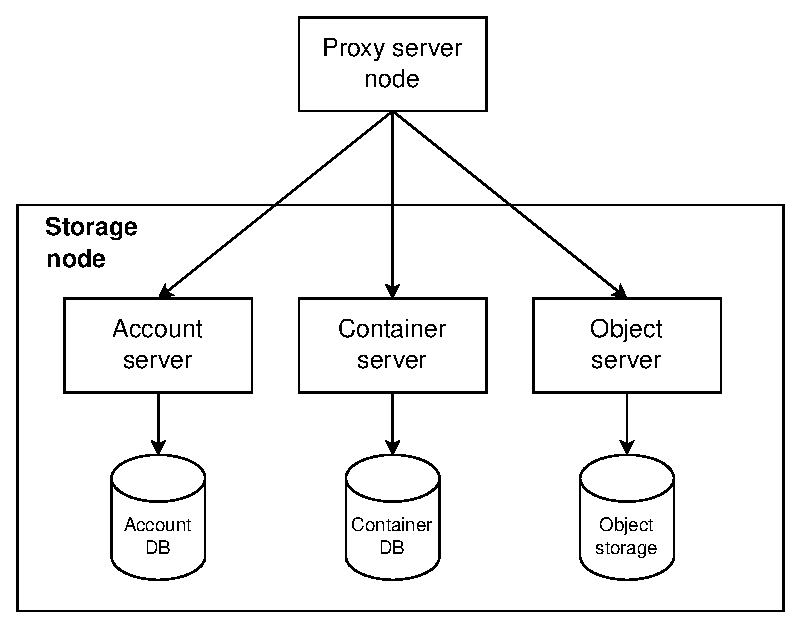
\includegraphics[width=0.75\textwidth]{obrazky-figures/swift-servers.eps}
        \caption{OpenStack Swift servers architecture.}
        \label{fig:beanstalkdJobSM}
    \end{figure}

    \section{Middlewares}
    Using Python WSGI middleware users can add functionalities and behaviors to OpenStack Swift. Most middlewares are added to the Proxy server, but can also be part of other servers (account server, container server or object server).

    Middlewares are added by changing configuration of servers. In example \ref{lst:swiftMiddleware}
    webhook middleware is added into proxy server by changing its pipeline (\textit{pipeline:main}). Middlewares are executed in given order (first will be called webhook middleware then proxy-server middleware).

    Some of the middlewares are required and will be automatically inserted by swift code\cite{swiftMiddleware}.

    \subsection{Interface}
    OpenStack Swift servers are implemented using Python WSGI applications. Therefore only Python WSGI middlewares are accepted in OpenStack Swift.

    In \ref{lst:swift-healthcheck} is example of simplified healthcheck middleware. Constructor takes two agruments, first is WSGI application and second is configuration of middleware defined using Python Paste framework in proxy-server.conf. Middlware must have call method, containing the request environment informations and response from previous called middleware. Middleware can preform some operations and call next middleware in pipeline, or inercept a request. In healtcheck example, if path directs to /healtcheck , middleware will return HTTP Response and other middlewares in pipeline will not be called.

    Method filter\_factory is used by Python Paste framework to instantiate middleware.

    \definecolor{codegreen}{rgb}{0,0.6,0}
    \definecolor{codegray}{rgb}{0.5,0.5,0.5}
    \definecolor{codepurple}{rgb}{0.58,0,0.82}
    \definecolor{backcolour}{rgb}{0.95,0.95,0.92}

\lstdefinestyle{mystyle}{
    backgroundcolor=\color{backcolour},
    commentstyle=\color{codegreen},
    keywordstyle=\color{blue},
    numberstyle=\tiny\color{codegray},
    stringstyle=\color{codepurple},
    basicstyle=\ttfamily\footnotesize,
    breakatwhitespace=false,
    breaklines=true,
    captionpos=b,
    keepspaces=true,
    numbers=left,
    showspaces=false,
    showstringspaces=false,
    showtabs=false,
    tabsize=2,
    caption=Example of healthcheck middleware in OpenStack Swift,
    label=lst:swift-healthcheck
}

\lstset{style=mystyle}

\begin{lstlisting}[language=Python]
import os
from swift.common.swob import Request, Response

class HealthCheckMiddleware(object):
    def __init__(self, app, conf):
        self.app = app

    def __call__(self, env, start_response):
        req = Request(env)
        if req.path == '/healthcheck':
            return Response(request=req, body=b"OK", content_type="text/plain")(env, start_response)
        return self.app(env, start_response)

def filter_factory(global_conf, **local_conf):
    conf = global_conf.copy()
    conf.update(local_conf)

    def healthcheck_filter(app):
        return HealthCheckMiddleware(app, conf)
    return healthcheck_filter
\end{lstlisting}

    \subsection{Metadata}
    OpenStack Swift separates metadata into 3 categories based on their use:
    \begin{itemize}
        \item \textbf{User Metadata} - User metadata takes form \textbf{X-<type>-Meta-<key>: <value>}, where \textbf{type} represent resource type(i.e. account, container, object), where \textbf{<key>} and \textbf{<value>} are set by user. User metadata remain persistent until are updated using new value or removed using header  \textbf{X-<type>-Meta-<key>} with no value or a header \textbf{X-Remove-<type>-Meta-<key>: <ignored-value>}.
        \item \textbf{System Metadata} - System metadata takes the form of \textbf{X-<type>-Sysmeta-<key>: <value>}, where \textbf{type} represent resource type(i.e. account, container, object) and \textbf{<key>} and \textbf{<value>} are set by internal service in Swift WSGI Server.
        All headers containing system metadata are deleted from client request.

        System metadata are visible only inside Swift provides mean to store potentially sensitive informations regarding Swift resources.
        \item \textbf{Object Transient-Sysmeta} - System metadata takes the form of \textbf{X-Object-Transient-Sysmeta-<key>: <value>}. Transient-sysmeta have similar behavior as system metadata, they can be access only within Swift and headers containing Transient-sysmeta are droped. If middleware want to store object metadata, it should use transient-sysmeta\cite{swiftMiddleware}.
    \end{itemize}


\chapter{MinIO}

\chapter{Solution draft}
\section{Current state}
    \subsection{OpenIO SDS}
    OpenIO Software-Defined storage has event-driven acrhitecture, capable of publishing events to Beanstalkd using \textit{event-agent service} and \textit{Notify filter}.
    Main disadvantage of current event publishing state is that configuration describing what type of events should be published is applied to whole storage. Since OpenIO SDS is multi-tenant space, some tenants might be interested in different events inside storage. The best use-case solution would be to let tenats decide what kind of events should be published in storage assigned to them.

    Second disadvantage is \textbf{lack of event filters}. Tenants might be interested in events involving specific objects or buckets that satisfy specific rules (for example object prefix, size, etc).

    Third disadvantage is that events are published only to beanstalkd queue. OpenIO SDS does not support any other destinations for event pubslishing. Since events can be used for monotoring, there should be proper interface, allowing users to define destionation for even pubslishing (i.e. Kafka, Prometheus, Grafana).

    \subsection{OpenStack Swift}
    Currently there is support for event pubslishing in OpenStack Swift. For example there is no way to detect changes in a given container except listing its content and comparing timestamps.

    To partialy solve this problem, OpenStack Swift created specification of middleware that would send out notifications to users if new object was created, metadata updated or or data has been deleted.
    There were two proposed solutions, both lacking common interface for event pubslishing (no support for either Amazon S3 or CloudEvents), which were not accepted and are outdated.

    \subsection{MinIO}
    MinIO supports event publishing in form of Bucket notifications. It can inform user when a object is created, updated or deleted. MinIO offers various notification targets (i.e. MySql, Redis, Elasticsearch) but does not offer Beanstalkd as notification target.

    MinIO provides only event pubslhing for buckets. There is no support for any events in account level (i.e. creating a new bucket, updating buckets metadata).

    Minio is open-source object storage but does not provide custom middlewares. Since MinIO is implemented is Go programming language, any custom changes (tweaks) in MinIO source code means that whole project needs to be compiled, which can result in uncompatibility in futures versions of MinIO.

\section{Middleware for OpenStack Swift and OpenIO SDS}
    The goal is to create common middleware that is capable of runing within OpenStack Swift aswell as OpenIO SDS. The middleware will allow user to configure: which types of events will be published and destionation where given events will be published.

    \subsection{Location}
    For OpenIO SDS ideal place to run new middleware is inside pipeline of event-agent. The main reasons is that event-agent has access to every event that occurs in OpenIO SDS and process jobs in asynchronous mode, which means it will not have impact on latency of clients requests.

    Most of middlewares within OpenStack Swift are placed in Proxy server, since they can react to every client request. Therefore, new proposed middleware will be placed inside proxy server pipeline.

    \subsection{Design}
    Middleware heavily utilizes containers/buckets and accounts metadata. Information about which event should be pubslished and where, will be stored stored in metadata of upper level. For publishing events regarding objects, configuration will be stored in a container/bucket metadata (for container/bucket events configuration will be stored in account level).

    Compared to Amazon S3 Notifications, EventNotification middleware will be capable of publishing events regarding containers/buckets. Futhermore, EventNotification middleware will be able to publish events regarding reading content from object storage (HTTP GET/HEAD), where Amazon S3 only offers notifications about changes (PUST/POST) in bucket.

    EventNotification middleware can be configured so that specific even types will be forbidden for publishing in whole object storage. In use case where could be a lot of reads from object storage, and publishing those events cound have big impact on object storage performance. Therefore such event types can be disabled for whole object storage.

    \paragraph{Event Notification configuration}

    \paragraph{Structure of published event}


    Activity diagram of EventNotification middleware in container level is shown in figure \ref{fig:middlewareActivity}. Container metadata contains event notification configration for publishing objects in given container. Therefore first step is to parse and validate such metadata. If the event notification configuration is not valid, then it is removed from metadata.

    Next step is deciding if event should be published. Since metadata about event publishing are stored in upper level, EventNotification needs to read account metadata from storage. After reading and parsing account metadata, EventNotification middleware checks if event satisfies rule in configuration retrieved from account metadata. If yes, then event will be published to specified destination in account metadata.

    \begin{figure}[hbt]
        \centering
        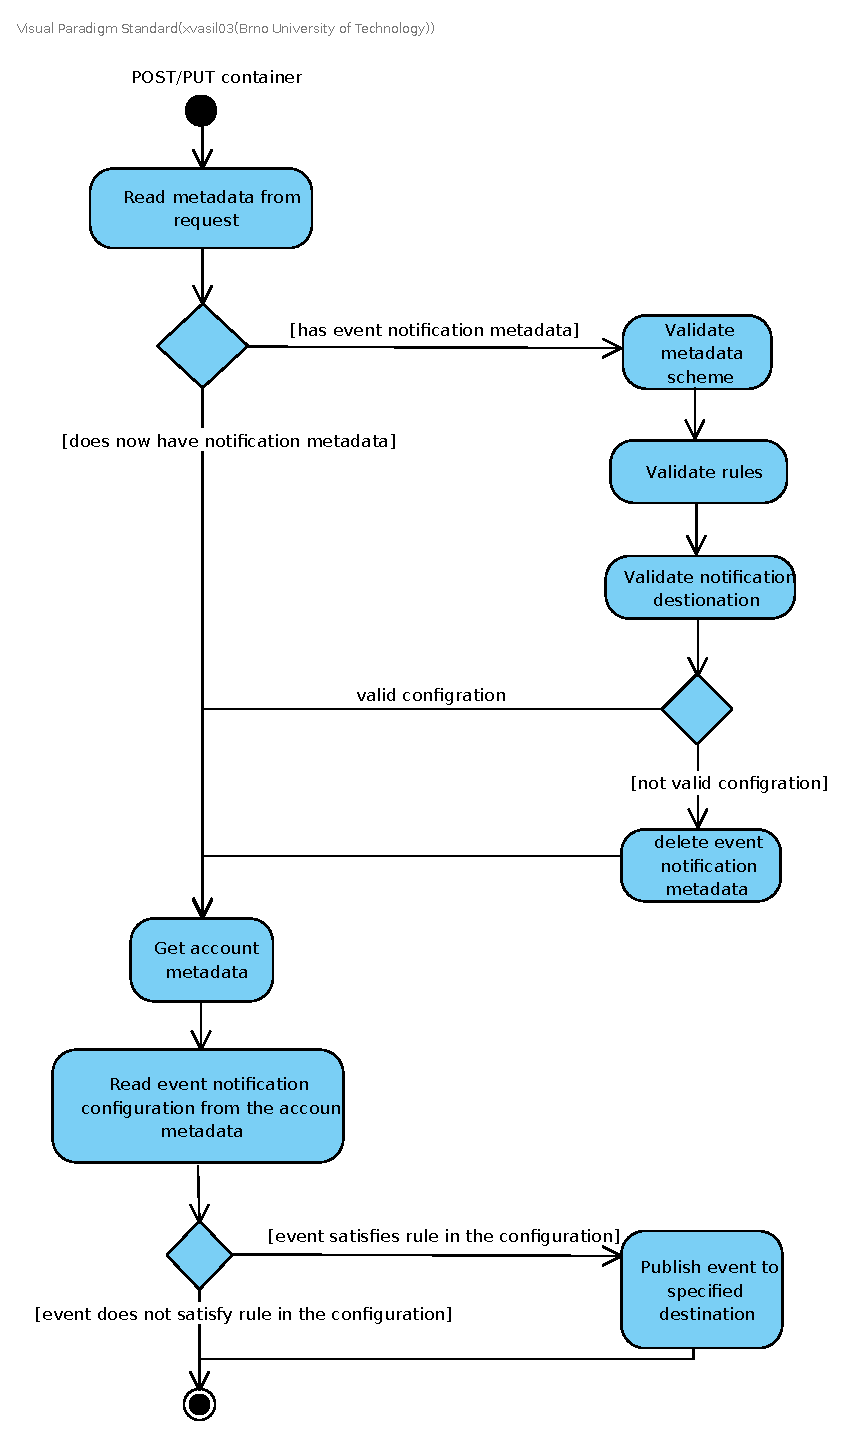
\includegraphics[width=0.8\textwidth]{obrazky-figures/middleware-activity-diagram.eps}
        \caption{Acitiviy diagram of EventNotification middleware.}
        \label{fig:middlewareActivity}
    \end{figure}



\section{Adapter for MinIO}
\chapter{Implementation, experiments and assessment}

\chapter{Conclusion}

%=========================================================================
